\subsection{Computational Performance} \label{sec:results-ssdtp}
In this subsection we investigate the scalability properties of the proposed solution for the SSDTP calculation and compare it with the approaches based on the FFT (\secref{sec:ssdta-analytical}), TTA with the analytical solution (\secref{sec:tta-analytical}), and TTA with HotSpot (\secref{sec:hotspot-iterative-solution})\footnote{All the experiments are performed on a Linux machine with Intel\textregistered\ Core\texttrademark\ i7-2600 3.4GHz and 8Gb of RAM.}. In the last two cases, the TTA is run until the normalized RMSE relative to the SSDTP obtained with the proposed method is less than 1\%.

In the following experiments, the sampling interval is set to \mbox{1 $ms$} and thermal configuration of the die is the same as in \tabref{tab:parameters}. The leakage modeling is not included in the results and will not affect the computational time in the case of the linearized model (\secref{sec:linearized-leakage}), whereas, the computational time using the iterative model (\secref{sec:iterative-leakage}) will be increased proportionally to the number of required iterations (due to the leakage power).

\iimage{scaling-time}{-100 0 -100 0}{Scalability with the application period for a quad-core architecture on the semilogarithmic scale.}

\begin{table}[t]
  \centering
  \caption{Performance comparison.}

  \subfloat[Scalability with the application period.]{
    \label{tab:scaling-time}
    \begin{tabular}{|r|r|r|r|r|}
      \hline
      $\period$, $s$ & $PM$, $ms$ & $FFT$, $\times$ & $TTA^{AS}$, $\times$ & $TTA^{HS}$, $\times$ \\
      \hline
      \hline
      0.05 & 0.18 & 52.12 & 168.71 & 6750.96 \\
      0.10 & 0.39 & 41.64 &  77.91 & 5301.97 \\
      0.20 & 0.67 & 41.64 &  42.79 & 5188.80 \\
      0.30 & 1.03 & 39.09 &  27.97 & 5030.25 \\
      0.40 & 1.36 & 39.16 &  21.43 & 4887.90 \\
      0.50 & 1.70 & 43.56 &  16.99 & 4880.57 \\
      0.60 & 2.04 & 40.86 &  14.34 & 4899.20 \\
      0.70 & 2.32 & 42.46 &  12.87 & 4935.89 \\
      0.80 & 2.66 & 41.70 &  11.07 & 4842.62 \\
      0.90 & 2.98 & 42.54 &  10.21 & 4883.76 \\
      1.00 & 3.33 & 45.19 &   9.23 & 4892.86 \\
      \hline
    \end{tabular}
  }

  \subfloat[Scalability with the number of cores.]{
    \label{tab:scaling-cores}
    \begin{tabular}{|r|r|r|r|r|}
      \hline
      $N_p$ & $PM$, $ms$ & $FFT$, $\times$ & $TTA^{AS}$, $\times$ & $TTA^{HS}$, $\times$ \\
      \hline
      \hline
       2 &  0.77 & 70.79 & 15.74 & 3236.75 \\
       4 &  1.63 & 46.09 & 17.68 & 2906.30 \\
       8 &  4.67 & 30.08 & 20.40 & 2695.69 \\
      16 & 15.48 & 21.08 & 24.36 & 2434.74 \\
      32 & 56.44 & 13.13 & 27.24 & 2214.19 \\
      \hline
    \end{tabular}
  }

\end{table}
First, we vary the application period $\period$ keeping the architecture fixed, which is a quad-core platform with the core area of 4 $mm^2$. The comparison is depicted in \figref{fig:scaling-time}. The computational time with the proposed method (PM) and its speed-up relative to the rest are given in \tabref{tab:scaling-time}. It can be seen that the proposed technique is roughly 5000 times faster than calculating the SSDTP by running the TTA with HotSpot ($TTA^{HS}$) and from 9 to 170 times faster than the TTA with the analytical solution ($TTA^{AS}$).

\iimage{scaling-cores}{-100 0 -100 0}{Scalability with the number of cores on the semilogarithmic scale.}
In the second experiment we evaluate the scalability of the proposed method with regard to the number of processing elements. The results are shown in \figref{fig:scaling-cores} and \tabref{tab:scaling-cores}. In can be observed that the proposed solution provides a significant performance improvement relative to its competitors where in order to keep the same level of accuracy the TTA requires larger number of periods of the application to be analyzed.

\subsection{Reliability Optimization} \label{sec:reliability-results}
In this section we evaluate the reliability optimization approach described in \secref{sec:reliability-problem} first with a set of hypothetical applications and, finally, using a real-life example.

The experimental setup is the following. Heterogeneous platforms and periodic applications are generated randomly \cite{dick1998} in such a way that the execution time of tasks is uniformly distributed between 1 and 10 $ms$ and the leakage power accounts for 30--60\% of the total power dissipation\footnote{The parameters of the applications and platforms (task graphs, floorplans, HotSpot configurations, etc.) used in our experiments are available at \cite{liu2011}.}. The linear leakage model is used in the experiments, since, as discussed in \secref{sec:linearized-leakage}, it provides a satisfactory approximation. The area of one core is 4 $mm^2$, other parameters of the die and thermal package are given in \tabref{tab:parameters}. The temperature constraint $T_{max}$ (see \equref{eq:t-max}) is set to $100^\circ C$. In \equref{eq:cycles-to-failure} the Coffin-Manson exponent $b$ is set to 6, the activation energy $E_a$ to 0.5, and the elastic temperature region $\Delta T_0$ to zero \cite{jedec2010}. The coefficient of proportionality $A$ is indifferent, since we are concerned about the relative improvement as described in the following.

In each of the experiments, we compare the optimized solution with an initial temperature-aware solution proposed in \cite{xie2006}. The solution is a combination of a task mapping and schedule that captures the spatial temperature behaviour and tries to minimize the peak temperature while satisfying the real-time constraints. This combination is the starting point for the future optimization. The deadline of the application is set to the duration of the initial schedule extended by 5\%.

\begin{table*}[t]
  \centering
  \caption{Results of the optimization.}
  \subfloat[Different number of cores.]{ \label{tab:mttf-cores}
    \begin{tabular}{|r|r|r|r|r|}
      \hline
      $N_p$ & $N_t$ & $t, s$ & $\mttfimp$ & $\eimp$ \\
      \hline
      \hline
      % 0% tolerance, 200-200-200-200-200 (mine)
      %  2 &   40 &     7.84 &  39.41 & 0.97 \\
      %  4 &   80 &    65.76 &  37.11 & 0.99 \\
      %  8 &  160 &   759.29 &  31.36 & 0.97 \\
      % 16 &  320 &  3484.59 &  13.51 & 0.98 \\
      % 32 &  640 &  7358.01 &   3.05 & 1.05 \\
      % 400 stall
      % 32 &  640 & 12732.54 &   3.82 & 1.05 \\

      % 0.5% tolerance, 200-200-200-400-400 (mine)
       2 &   40 &     5.51 &  50.99 & 0.98 \\
       4 &   80 &    34.27 &  39.95 & 0.98 \\
       8 &  160 &   278.81 &  28.28 & 0.93 \\
      16 &  320 &  2203.77 &   8.38 & 0.99 \\
      32 &  640 & 12732.54 &   3.82 & 1.05 \\
      \hline
    \end{tabular}
  }
  \subfloat[Different application sizes.]{ \label{tab:mttf-tasks}
    \begin{tabular}{|r|r|r|r|r|}
      \hline
      $N_p$ & $N_t$ & $t, s$ & $\mttfimp$ & $\eimp$ \\
      \hline
      \hline
      % 0% tolerance, 200-200-200-200-200 (Min)
      % 4 &  40 &   9.96 & 64.53 & 0.88 \\
      % 4 &  80 &  56.57 & 38.01 & 0.96 \\
      % 4 & 160 & 352.20 & 18.08 & 1.07 \\
      % 4 & 320 & 408.42 & 12.92 & 1.05 \\
      % 4 & 640 & 222.46 &  3.90 & 1.03 \\
      % 1000 stall
      % 4 & 640 & 1042.86 & 5.60 & 1.03 \\

      % 0.5% tolerance, 200-300-400-500-600 (Sergiu)
      % 4 &  40 &    6.49 & 121.54 & 0.93 \\
      % 4 &  80 &   34.32 &  51.80 & 0.97 \\
      % 4 & 160 &  150.61 &  39.90 & 1.03 \\
      % 4 & 320 &  426.93 &   6.55 & 1.07 \\
      % 4 & 640 &  519.22 &   3.75 & 1.03 \\

      % 0.5% tolerance, 200-200-300-500-1000 (Sergiu)
      4 &  40 &    8.38 & 61.46 & 0.89 \\
      4 &  80 &   31.03 & 36.79 & 0.94 \\
      4 & 160 &  131.90 & 29.44 & 0.99 \\
      4 & 320 &  514.15 &  6.51 & 1.07 \\
      4 & 640 & \todo{0} & 3.75 & 1.03 \\
      \hline
    \end{tabular}
  }
  \subfloat[Different techniques.]{ \label{tab:mttf-comparison}
    \begin{tabular}{|r|r|r|r|r|}
      \hline
      $N_p$ & $N_t$ & $\mttfimp^{PM}$ & $\mttfimp^{HS}$ & $\mttfimp^{SSA}$ \\
      \hline
      \hline
      4 &  40 & 61.46 & 1.29 & 25.10 \\
      4 &  80 & 36.79 & 1.67 & 13.87 \\
      4 & 160 & 29.44 & 2.02 &  5.33 \\
      4 & 320 &  6.51 & 1.72 &  3.81 \\
      4 & 640 &  3.75 & 1.20 &  \todo{0} \\
      \hline
    \end{tabular}
  }
\end{table*}

In the first set of experiments, we change the number of cores $N_p$ while keeping the number of tasks $N_t$ per core constant and equal to 20. For each problem we have generated 20 random task graphs and found the average improvement of the MTTF. We also have measured the change in the consumed energy. The results are given in \tabref{tab:mttf-cores}. It can be seen that the reliability-aware optimization dramatically increases the MTTF by 4 up to 50 times ($\mttfimp$). The improvement decreases with the growth of the number of cores and total number of tasks. However, even for large applications with, e.g., 320 tasks deployed onto 16 cores a feasible mapping and schedule that significantly improve the lifetime of the system can be found in a reachable time. Moreover, our reliability optimization does not impact the energy efficiency of the system. On the contrary, as it can be seen from \tabref{tab:mttf-cores}, the result of the optimization is a decrease in the energy consumption ($\eimp$).

For the second set of experiments, we keep the quad-core architecture and vary the size (number of tasks $N_t$) of the application. The number of randomly generated task graphs per application size is 20. The average improvement of the MTTF ($\mttfimp$) along with the change in the energy consumption ($\eimp$) are given in \tabref{tab:mttf-tasks}. The observations to be made here are similar to the previous ones: reliability optimization, during the design stage, can significantly prolong the MTTF without sacrificing the energy efficiency of the system.

The above experiments have confirmed that our proposed approach is able to effectively increase the MTTF of the system and, at the same time, reduce its energy consumption. The efficiency of this approach is due to the fast and accurate SSDTP calculation, which is the heart of the optimization, and which, due to its speed, allows a huge portion of the design space to be explored. In order to prove this, we have replaced, inside our optimization framework, the proposed SSDTP calculation with the calculation based on HotSpot (\secref{sec:hotspot-iterative-solution}) and based on the SSA (\secref{sec:steady-state-approximation}), respectively. The computation of the SSDTP with HotSpot is stopped when the maximal difference between two successive iterations is less than $0.01^\circ C$ or the limit of 30 iterations is reached (although, it is not sufficient for a good accuracy as it is shown in \secref{sec:hotspot-iterative-solution}). The experimental setup is the same as for the experiments in \tabref{tab:mttf-tasks}. The optimization procedure of each task graph is limited by the same time that the proposed approach has taken to perform it. The final solutions found by HotSpot and the SSA are reevaluated using our method and compared with the solutions found only by the proposed technique ($\mttfimp^{PM}$). The results are summarized in \tabref{tab:mttf-comparison} where the reevaluated solutions are denoted as $\mttfimp^{HS}$ and $\mttfimp^{SSA}$, respectively. In can be seen that the proposed technique outperforms its competitors. For instance, the lifetime of the platform running 160 tasks can be extended by around 30 times using our approach, whereas, the best solutions found by HotSpot and the SSA are only 2.02 and 5.33, respectively.

We have seen that our reliability-targeted optimizations have significantly increased the MTTF without affecting the energy consumption. This is not surprising, since our optimization will search towards low temperature amplitudes, which implicitly means low leakage. In order to further explore this aspect, we have performed a multi-objective optimization\footnote{The multi-objective optimization is based on the NSGA-II algorithm \cite{deb2002}.} along the dimensions of energy and reliability. An example of the Pareto front averaged over 20 applications with 80 tasks deployed onto a quad-core platform is given in \figref{fig:average-pareto}. It can be observed that the variation of energy is less than 2\%. This means that solutions optimized for the MTTF have an energy consumption almost identical to those optimized for energy. At the same time, the difference of the MTTF is extremely huge. This means that ignoring the reliability aspect one may end up with a significantly decreased the MTTF without any significant gain in terms of energy.
\begin{figure}[b]
  \centering
  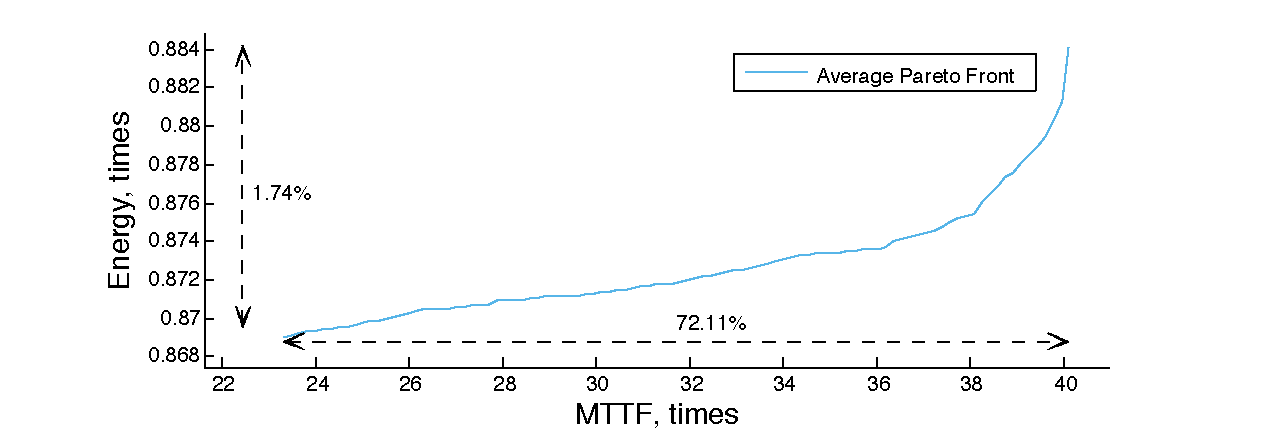
\includegraphics[width=1.0\linewidth]{assets/average-pareto.pdf}
  \caption{The average Pareto front.}
  \label{fig:average-pareto}
\end{figure}

Finally, we have applied our optimization technique to a real-life example, namely the MPEG2 video decoder \cite{ffmpeg2011} that is deployed onto a dual-core architecture. The decoder was analysed and split into 34 tasks. The parameters of each task were obtained through a system-level simulation on the MPARM platform \cite{benini2005}. The deadline is set to 40 $ms$ assuming 25 video frames per second. The solution found by the GA with the proposed method improves the lifetime of the system 23.59 times with a 5\% energy saving. The same optimization problem was solved using the TTA with HotSpot and SSA as it is described earlier. The best found solutions are 5.37 and 11.50, respectively.
